\documentclass[tikz,border=10pt]{standalone}
\usepackage{tikz}
\begin{document}
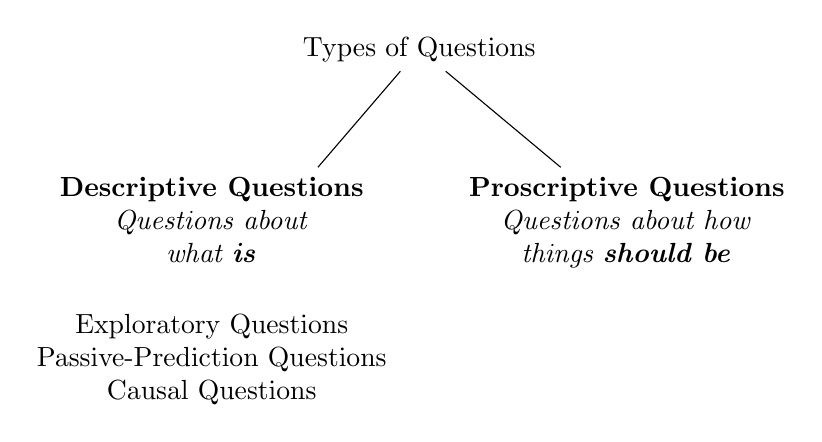
\begin{tikzpicture}[
  sibling distance=15em,
  every node/.style = {align=center, anchor=north}]]
  \node {Types of Questions}
    child { node {\textbf{Descriptive Questions} \\ \emph{Questions about} \\ \emph{what \textbf{is}} \\ \vspace{.05cm} \\ Exploratory Questions \\ Passive-Prediction Questions \\ Causal Questions} }
    child { node {\textbf{Proscriptive Questions} \\ \emph{Questions about how} \\ \emph{things \textbf{should be}}} };
\end{tikzpicture}
\end{document}